\begin{enunciado}
 Se supone que una m\'aquina mezcla cacahuates, avellanas, anacardos y pacanas
 a raz\'on de $5:2:2:1$.
 Se encuentra que una lata que contiene $500$ de tales nueces mezcladas tiene
 $269$ cacahuates, $112$ avellanas, $74$ anacardos y $45$ pacanas.
 Al nivel de significancia de $0.05$, pruebe la hip\'otesis
 de que la m\'aquina mezcla las nueces a una raz\'on de $5:2:2:1$.
\end{enunciado}

\begin{solucion}
 Para la soluci\'on, se va a definir una variable aleatoria $X$,
 que es una codificaci\'on de las nueces como $1,2,3$ y $4$
 para los cacahuates, las avellanas, los anacardos y las pecanas,
 respectivamente.
 As\'{\i}, pues, probar que la m\'aquina mezcla las nueces a una proporci\'on
 $5:2:2:1$ es equivalente a probar que $X$ sigue una distribuci\'on
 cuyos valores est\'an asignados como
 $f(x) = \frac{f_x}{f_1+f_2+f_3+f_4}$,
 para cada $x\in\mathbb{N}\cap[1,4]$ donde $f_X$
 es la frecuencia esperada, es decir,
 en este caso que se espera una raz\'on $5:2:2:1$, se puede 
 considerar $f_1=5$, $f_2=2$, $f_3=2$ y $f_4=1$,
 por lo que $f_1+f_2+f_3+f_4=5+2+2+1=10$ y
 $f(1)=\frac{5}{10}=\frac{1}{2}$,
 $f(2)=f(3)=\frac{2}{10}=\frac{1}{5}$
 y $f(4)=\frac{1}{10}$. 
 \begin{datos}
  $\phantom{0}$
  \begin{itemize}
   \item Tama\~no de la muestra: $n=500$.
   \item Frecuencias observadas:
   $O = \{ o_1 = 269, o_2 = 112, o_3 = 74, o_4 = 45 \}$.
   \item Probabilidades esperadas: $p_1 = \frac{1}{2}$,
   $p_2 = \frac{1}{5}$, $p_3 = \frac{1}{5}$ y $p_4 = \frac{1}{10}$
   \item frecuencias esperadas:
   $E = \left\{ e_i=n\cdot p_i \, | \forall\, i\in\mathbb{N}\cap[1,4] \right\} = \{ e_1 = 250, e_2 = 100, e_3 = 100, e_4 = 50 \}$.
   \item Celdas totales del experimento: $k=4$.
   \item Grados de libertad de la prueba $\chi^2$: $v = k-1 = 3$.
  \end{itemize}
 \end{datos}

 \begin{hipotesis}
  Prueba de bondad de ajuste para probar $H_0:$
  que una variable aleatoria $X$ de $4$ valores sigue una distribuci\'on
  con una raz\'on de $5:2:2:1$,
  contra la alternativa $H_1$ de que no es as\'{\i}.
 \end{hipotesis}

 \begin{estadistico}
  \begin{eqnarray*}
   \chi^2 & = & \sum_{i=1}^k \frac{\left( o_i - e_i \right)^2}{e_i}
   =\frac{(269 - 250)^2}{250} + \frac{(112 - 100)^2}{100} +
   \frac{(74-100)^2}{100} + \frac{(45-50)^2}{50} \\
   & = & \frac{19^2}{250} + \frac{12^2}{100} + \frac{26^2}{100} +
   \frac{5^2}{50}
   = \frac{361(2) + 144(5) + 676(5) + 25(10)}{500} = \frac{5\,072}{500}\\
   & = & \frac{1\,268}{125} = 10.144
  \end{eqnarray*}
 \end{estadistico}

 \begin{valorp}
  De la tabla A.5 se observa que $\chi^2_{0.02,3} \approx 9.837$
  $\chi^2_{0.01,3} \approx 11.345$,
  entonces, como $\chi^2_{0.02,3} < \chi^2 < \chi^2_{0.01,3}$,
  se sigue que el $P-$valor es un valor aproximadamente de $0.015$.
 \end{valorp}

 \begin{conclusion}
  Como el valor $P$ es muy peque\~no,
  se concluye que la muestra presentada es evidencia suficiente
  para rechazar la hip\'otesis nula y, por lo tanto, afirmar
  que la raz\'on en que la m\'aquina mezcla las nueces no es $5:2:2:1$.
 \end{conclusion}

 En el c\'odigo registrado en el archivo
 \texttt{P16\_Prueba\_de\_bondad\_chi2\_02.r}
 se realiza este procedimiento.
 El c\'odigo permite modificar los valores iniciales que corresponden a:
 \texttt{datos} que guarda los datos de la lectura de un archivo, en este caso se lee el archivo
 \texttt{DB17\_Problema\_081.csv},
 y este \'ultimo nombre es el que se modifica para leer otros archivos;
 \texttt{varInteres} para indicar el nombre de la columna
 que corresponde a los datos, agrupados ya en celdas
 y que, por lo tanto, aparece cada valor una \'unica vez en dicha columna;
 \texttt{varFrecuencia} para indicar el nombre de la columna
 de la frecuencia observada correspondiente a cada valor;
 \texttt{varProb} que indica el nombre de la columna
 que contiene la probabilidad esperada para cada valor;
 \texttt{combinar} para indicar, con \texttt{TRUE}, que,
 si la frecuencia esperada en alguna celda es menor a $5$,
 se combinen celdas, y aunque se puede indicar con \texttt{FALSE}
 que no se realice este proceso, el no realizarlo puede dar un error,
 por lo que es recomendarlo mantenerlo en \texttt{TRUE};
 \texttt{grafica} para indicar, con \texttt{TRUE}, que se realizar\'a
 una gr\'afica comparando las proporciones observadas
 de las probabilidades esperadas, o \texttt{FALSE}
 en caso de no graficar;
 \texttt{tituloEjeX} para indicar el t\'{\i}tulo en el eje X
 cuando se realice una gr\'afica;
 y, \texttt{alfa} para el nivel de confianza.
 \par 
 El programa espera al menos los datos correspondientes a la base de datos,
 escrito en un archivo \texttt{.csv} con una columna con los datos 
 correspondientes a los valores de las celdas, la frecuencia de cada valor
 y la probabilidad esperada para cada valor.
 \par 
 Este programa es una versi\'on resumida
 de \texttt{P16\_Prueba\_de\_bondad\_chi2\_02.r},
 en el que ahora se espera siempre los datos resumidos en celdas,
 adem\'as de requerir en la base de datos las probabilidades
 esperadas en vez de una distribuci\'on, permitiendo mayor robustes.
 Por otro lado, para la gr\'afica que realiza el programa
 se requiere del paquete \texttt{MASS}.
 \par 
 El resultado muestra lo siguiente:
 \texttt{Variable} que indica el nombre y unidad de lo que se est\'a midiendo;
 \texttt{Estad\'{\i}stico Chisq2} para el valor del estad\'{\i}stico
 $\chi^2$;
 \texttt{Grados de libertad} para indicar la cantidad de grados de libertad
 usado en los c\'alculos de probabilidades de la disitribuci\'on $\chi^2$;
 \texttt{Valor-p} para indicar el $p-$valor;
 \texttt{alpha} que muestra el valor asignado en la variable \texttt{alfa},
 \'o $0.05$ en caso de que se le haya asignado \texttt{NULL};
 \texttt{Región de Rechazo} que indica a partir de cu\'al valor
 del estad\'{\i}stico se rechaza la prueba,
 seg\'un el valor \texttt{alpha} mostrado;
 y, adem\'as, si se ha indicado un valor a la variable \texttt{alfa},
 entonces aparece \texttt{Resultado} para indicar si se rechaza
 o no la hip\'otesis nula.
 \par 
 El c\'odigo junto con el resultado se muestra a continuaci\'on:
 \begin{verbatim}
> require(MASS)
> datos<-read.csv("DB17_Problema_081.csv",sep=";",encoding="UTF-8")
> varInteres<-"Mezcla.nueces"
> varFrecuencia<-"Frecuencia"
> varProb<-"Probabilidad"
> combinar<-TRUE
> grafica<-TRUE
> tituloEjeX<-"Mezcla de varios tipos de nueces"
> alfa<-NULL
> valores<-datos[,varInteres]
> frecObs<-datos[,varFrecuencia]
> probEsp<-datos[,varProb]
> colapsar<-function(p1,f1,lim1=5){
+   np1<-p1
+   nf1<-f1
+   tocollapse<-which((np1*sum(nf1))<lim1)
+   while(length(tocollapse)>0){
+     x<-tocollapse[1]
+     if (x<length(np1)){
+       np1[x+1]<-p1[x]+p1[x+1]
+       nf1[x+1]<-f1[x]+f1[x+1]
+     }else{
+       np1[x-1]<-p1[x]+p1[x-1]
+       nf1[x-1]<-f1[x]+f1[x-1]
+     }
+     p1<-np1[-x]
+     f1<-nf1[-x]
+     np1<-p1
+     nf1<-f1
+     tocollapse<-which((p1*sum(f1))<lim1)
+   }
+   return(list(probs=p1,freqs=f1))  
+ }
> calculos<-function(frecObs,probEsp,alfa=0.05){
+   if(length(frecObs)>1){
+     r<-NULL
+     if(combinar){
+       r1<-colapsar(probEsp,frecObs)
+       frecObsC<-r1$freqs
+       probEspC<-r1$probs
+       if(length(frecObsC)>1){
+         prueba<-chisq.test(frecObsC,p=probEspC)
+       }else{
+         prueba<-NA
+       }
+     }else{
+       prueba<-chisq.test(frecObs,p=probEsp)
+     }
+     if(!is.na(prueba[1]) & prueba$parameter > 0){
+       r<-c(prueba$statistic, prueba$parameter,prueba$p.value,alfa,
+            qchisq(alfa,prueba$parameter,lower.tail=FALSE))
+     }
+     if(is.null(r)){
+       r<-rep(NA,5)
+     }
+     return(r)
+   }
+ }
> if(!is.null(alfa)){
+   tabla<-t(as.matrix(calculos(frecObs,probEsp,alfa)))
+ }else{
+   tabla<-t(as.matrix(calculos(frecObs,probEsp)))
+ }
> tabla<-data.frame(nombre=varInteres,tabla)
> names(tabla)<-c("Variable","Estadístico Chisq2",
+                 "Grados de libertad","Valor-p","alpha","Región de Rechazo")
> tabla["Región de Rechazo"]<-paste(">",round(tabla["Región de Rechazo"],7))
> generaGrafica<-function(valores,frecuencia,probEspG,tituloEjeX,nomVariable){
+   x<-c()
+   for(i in 1:length(valores)){
+     x<-c(x,rep(valores[i],frecuencia[i]))
+   }
+   maxD<-max(density(x)$y)
+   x11()
+   probEspG<-c(probEspG,0)
+   truehist(x,h=1,
+            main=paste("Comparación de distribuciones","\n","Específica"),
+            xlab=tituloEjeX, ylab="Densidad",sub=nomVariable,
+            xlim=c((min(x)-1),(max(x)+2)),
+            ymax=max(max(probEspG),maxD)*1.2)
+   lines((min(x)):(max(x)+1),probEspG,type="s",col="red",lty=2,lwd=2)
+   legend("topleft",legend = c("Dist. original", "Dist. teórica"),
+          lwd=c(1,2),lty=2,col=c("black","red"))
+   invisible()
+ }
> if(!is.null(alfa)){
+   tabla$alpha<-alfa
+   tabla$Resultado<-ifelse(tabla$"Valor-p">=alfa,
+                          "No se rechaza el ajuste de bondad",
+                          "Se rechaza el ajuste de bondad")
+ }
> tabla
       Variable Estadístico Chisq2 Grados de libertad    Valor-p alpha
1 Mezcla.nueces             10.144                  3 0.01738092  0.05
  Región de Rechazo
1       > 7.8147279
> if (grafica){
+   generaGrafica(valores,frecObs,probEsp,tituloEjeX,varInteres)
+ }
 \end{verbatim}
 \vspace{-0.5cm}
 que incluye la siguiente figura:
 \begin{center}
  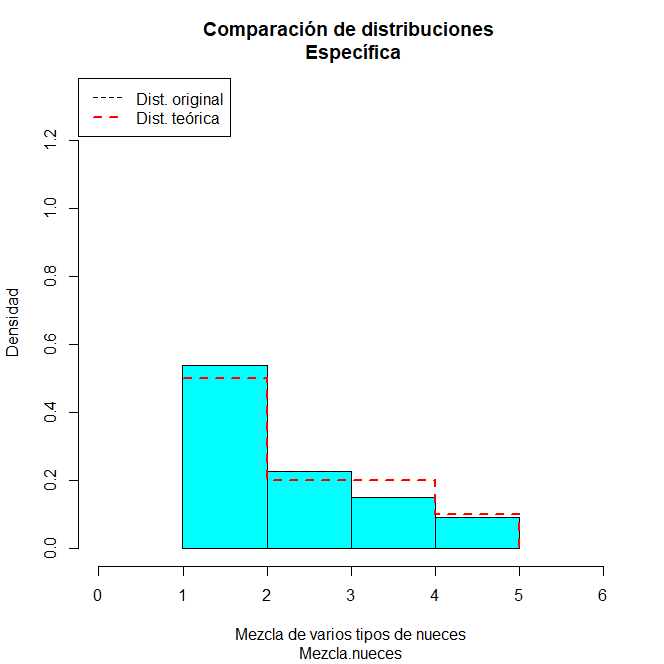
\includegraphics[scale=0.35]{Problema_81.png}
 \end{center}
 Lo cual coincide con los resultados obtenidos,
 que es a lo que se quer\'{\i}a llegar.${}_{\blacksquare}$
\end{solucion}
